\ifdefined\XeTeXrevision\else\pdfoutput=1\fi
\documentclass[11pt]{article}
\usepackage[margin=1in]{geometry}
\usepackage{booktabs}
\usepackage{amsmath}
\usepackage{graphicx}
\usepackage{xcolor}
\usepackage{hyperref}
\usepackage{microtype}
\hypersetup{colorlinks=true, linkcolor=blue!60!black, citecolor=blue!60!black,
  urlcolor=blue!60!black, pdftitle={The Host Is Part of the Block},
  pdfauthor={Franci Penov}}
\title{The Host Is Part of the Block:\\A Goal-Pursuit Ladder at Two Scales\\and the Composition-Matching Law}
\author{Franci Penov \\ kortexa.ai \\ \texttt{francip@kortexa.ai}}
\date{2026-08-11 (v1); revised 2026-08-15 (v2)}

\begin{document}
\maketitle

\begin{abstract}
The cadence notes~\cite{penov2026carrier,penov2026writer} left a goal
living in a conditioning channel and a creature-scale loop that holds
it; this note makes the goal DO something. A registered ladder (G0-G3
plus a temporal-pressure rung) puts a frozen host on a chained-clue
errand --- look, open, submit, under a tick budget, with every
episode's actions and observations recorded as first-class transcripts
--- at 230M with the validated activation-packet channel and at 27B
with the validated weight-block channel. Three findings. First, the
scale answer: zero-shot, BOTH hosts are below the task (0.00 with the
goal in text); trained by 384 steps of oracle cloning, both are perfect
when the goal rides in text (1.00 at every seed, both venues); trained
with the goal in the channel, both carry a partial want
(0.70/0.80/1.00 at 230M, 0.60/0.80/0.70 at 27B) that
directs behavior without surviving symbol-level conflict --- the
interesting gap is channel-vs-text, not small-vs-large. Second, the
environment fought the preregistration three times --- a reveal-order
leak, a mis-specified control floor, a Markovian degeneracy --- and the
registered controls caught all three; the diagnosis runs are kept.
Third, and the note's title: a conditioning artifact works exactly on
the host composition it was trained under --- and this revision can
state the law symmetrically, because its registered re-runs completed
both directions. At 230M the GT policy bridge scores 1.00 under the
host it trained under and 0.00 under any other, seat for seat: trained
dream4-only, the text arms are perfect and the temporal arm dead;
retrained under the temporal-armed host, the table inverts exactly,
and the swap reproduces at T=4 with fresh bridges. The serving
boundary obeys the same law: the trained errand policy first reached
0.40 through the real serving path --- read, wrongly, as the serve
wrapper's cost --- until the diagnosis that the isolated instance's
one block was never fed, so the server presents a BARE host; retrained
under that bare host, the same policy scores 1.00 through the
identical wrapper, cached-generate path, and byte-identical template.
The transfer gap was the training host both times; the serve wrapper
costs nothing; the operator mismatch (harness addition vs server
factor averaging, independently documented in the serving stack's own
audit) remains the one live defect for multi-block serving. And the
law's payoff rung follows it home: with per-arm host matching, a
temporal block carrying no time words gives the frozen 230M the same
wall-timed behavior under a hidden, noisy budget that a countdown
sentence gives it --- frozen-time and shuffled-time controls both at
the no-signal baseline --- the program's first time-feeling positive.
\end{abstract}

\section{From a want that persists to a want that acts}

Paper 12 measured a goal packet that endures; paper 13 closed its
re-encoding gap. The registered goal-pursuit line asks the next
question: can the want DRIVE something --- a multi-step errand through
tools --- and where does the want have to live for that to work? The
environment is deliberately small and fully machine-validated: eight
places, eight items, three-hop clue chains (a note names the next
place, the last place holds the target beside a generator-drawn
distractor, submit ends the episode), a tick budget of eight, greedy
decode, and a transcript for every episode. The distractor makes the
final submit a forced choice only the goal can decide; the oracle needs
four ticks. Venues: the 230M creature stack (dream4 armed, the
activation-packet channel the C-line validated) and the bare 27B column
(the weight channel the multi-sensor line validated) --- per-venue
channels, registered as such, because the claim is about WHERE the want
lives, not one mechanism.

\section{The environment fought back, and the controls won}

Three times the preregistered design was wrong, and three times its own
control cells said so before any claim shipped. The first G1 run scored
1.00 everywhere INCLUDING the goal-free floor whose submit is a coin
flip by construction --- the reveal listed the target first, and every
trained arm had learned ``submit the first-listed item.'' The floor
cell and the shuffled control caught it; the order is now randomized;
the leak run is kept as the diagnosis. The shuffled check itself was
then found mis-specified (registered against an untrained floor any
trained policy beats) and re-registered against the trained goal-free
floor. And G2's truncation rung returned its registered reading (iii):
each clue names the next move, so the errand is Markovian and
last-observation context recovers full performance exactly --- the rung
cannot separate state carriers on this task shape, recorded as a
task-design note. Its one live cell: a goal entering the packet once
and surviving on-policy re-encoding lands at 0.60/0.50/0.60 ---
direction above chance, weaker than text.

\section{The scale answer}

Table~\ref{tab:g1} and Figure~\ref{fig:hostlaw} (left) carry it.
Zero-shot, the errand defeats both hosts --- 0.00 success with the goal
stated in text, at 230M and at 27B alike (the 27B's transcripts do not
even wander well). Trained by oracle cloning with the goal in text,
both hosts are perfect: 1.00 at every seed, both venues. Trained with
the goal ONLY in the channel, both venues land in the same band ---
0.70/0.80/1.00 at 230M through the activation packet,
0.60/0.80/0.70 at 27B through the weight block --- above their
trained goal-free floors, below their text ceilings, and in
packet-vs-context conflict cells the channel's item is almost never
what gets submitted. The channel carries direction, not symbols, at
both scales; scale bought nothing on the channel; and the question the
program inherits is not ``is the model big enough'' but ``what does a
channel have to be for a want to survive contact with language.''

\begin{table}[t]
\centering
\small
\setlength{\tabcolsep}{5pt}
\begin{tabular}{lrrrr}
\toprule
venue & trained text & goal block & block done-choice & no-goal floor \\
\midrule
230M (activation packet) & 1.00/1.00/1.00 & 0.70/0.80/1.00 & 0.70/0.89/1.00 & 0.60/0.80/0.70 \\
27B (weight block) & 1.00/1.00/1.00 & 0.60/0.80/0.70 & 0.60/0.80/0.70 & 0.50/0.50/0.80 \\
\bottomrule
\end{tabular}
\caption{G1 at both venues, per seed. Both channels carry a partial
want; text carries a whole one; the floors are the trained goal-free
bridges whose submit is a coin flip.}
\label{tab:g1}
\end{table}

\section{The composition-matching law}

Four independent cells, one law: \emph{a conditioning artifact works
on the host composition it was trained under, and on no other.}
(1)~GT at 230M: a policy bridge trained on the dream4-only host scores
1.00 --- and 0.00 the moment the production temporal block's delta is
summed underneath it at evaluation
(none/countdown/temporal = 1.00/1.00/1.00 /
1.00/1.00/1.00 /
0.00/0.00/0.00).
(2)~GT at 27B reproduces the shape
(0.00/1.00/0.00 on the temporal arm).
(3)~The serving canary: the same emitter that passes its C1 gate
in-harness passes through the production server's cached-generate
delivery path on a matched dream4-only host --- true
0.60 against floors 0.20 and
0.00 --- validating the delivery wiring end to
end. (4)~Arm one more block and the same canary collapses to chance
(0.20), even for an emitter retrained under the
moving temporal host; the residual mismatch is the OPERATOR: the
harness composes blocks by flat-delta addition, the server by LoRA
factor averaging with cross-terms --- a bug the serving stack's own
audit had independently documented. Two investigation lines, one root
cause; the fix pays both. (5)~The registered re-run makes the first
cell symmetric: the same recipe with the regime bridge trained under
the temporal-armed host inverts Table~\ref{tab:gt} exactly ---
temporal 1.00/1.00/1.00 on the oracle path, none and countdown
0.00/0.00/0.00 with $\sim$50 invalid actions per cell --- and a T=4
closure pair reproduces the swap seat for seat with freshly trained
bridges (Table~\ref{tab:gtswap}); train/serve host match fully
determines the outcome in both directions. (6)~The serving boundary's
re-run closes cell (3)'s residue the same way
(Section~\ref{sec:serve}). The law's constructive corner: the emitter
retrained under the moving host keeps its write-once packets at
0.97--1.00 across sixteen ticks (1.00 early,
0.97 late), while its live re-encoding loop
degrades (0.55/0.25) ---
the store architecture is robust where the self-loop is not.

\begin{table}[t]
\centering
\small
\begin{tabular}{lrrr}
\toprule
venue & none & countdown & temporal block \\
\midrule
230M & 1.00/1.00/1.00 & 1.00/1.00/1.00 & 0.00/0.00/0.00 \\
27B & 1.00/1.00/1.00 & 1.00/1.00/1.00 & 0.00/1.00/0.00 \\
\bottomrule
\end{tabular}
\caption{GT per seed: the text arms are ceilinged (the trained policy
is oracle-optimal, so the tight budget exerts no pressure) and the
temporal arm measures host mismatch, not time-feeling --- the bridge
never trained under the summed host. The re-run that trains under it
inverts the table (Table~\ref{tab:gtswap}).}
\label{tab:gt}
\end{table}

\begin{table}[t]
\centering
\small
\begin{tabular}{llrrr}
\toprule
budget & regime bridge trained under & none & countdown & temporal \\
\midrule
T=5 & dream4-only (original) & 1.00/1.00/1.00 & 1.00/1.00/1.00 & 0.00/0.00/0.00 \\
T=5 & dream4+temporal (re-run) & 0.00/0.00/0.00 & 0.00/0.00/0.00 & 1.00/1.00/1.00 \\
T=4 & dream4-only & 1.00/1.00/1.00 & 1.00/1.00/1.00 & 0.00/0.00/0.00 \\
T=4 & dream4+temporal & 0.00/0.00/0.00 & 0.00/0.00/0.00 & 1.00/1.00/1.00 \\
\bottomrule
\end{tabular}
\caption{The GT-230M swap, per seed: train/serve host match fully
determines the outcome in both directions, at two budgets, with
freshly trained bridges each time. Every matched cell runs the oracle
path (mean done-tick 4.0 flat); every mismatched cell emits invalid
actions until the budget dies.}
\label{tab:gtswap}
\end{table}

\begin{figure}[t]
\centering
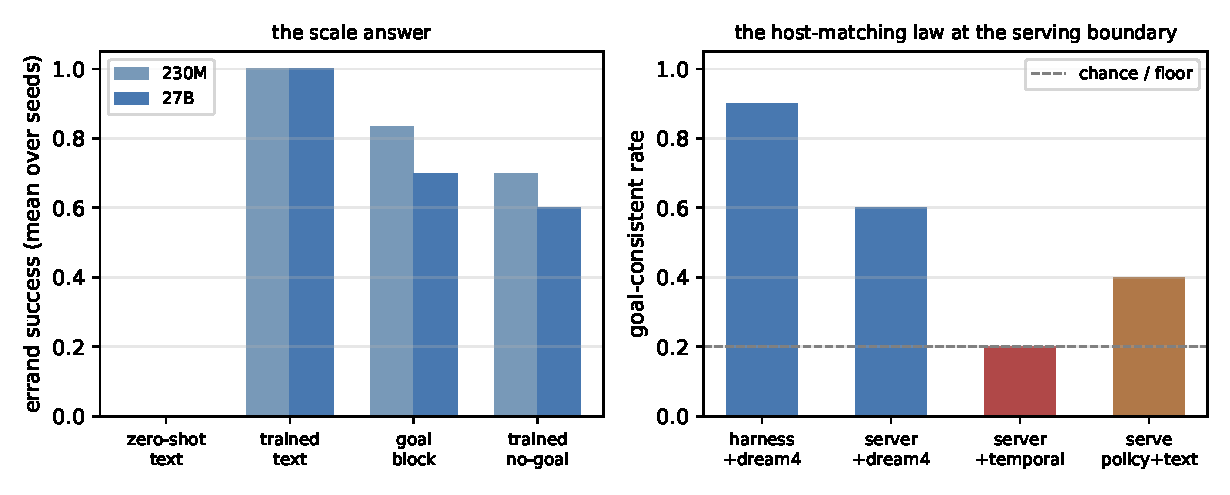
\includegraphics[width=\linewidth]{host-law.pdf}
\caption{Left: the scale answer --- zero-shot below task, trained-text
perfect, channel partial, at both venues. Right: the law at the
serving boundary --- the same artifacts pass on matched hosts
(harness+dream4, server+dream4), collapse under one extra block
(server+temporal, the operator mismatch), and the trained policy
delivered through the real serving path reaches
0.40 against a 1.00 harness ceiling --- a gap the bare-host retrain
closes to 1.00 (Section~\ref{sec:serve}); the figure keeps the v1
number as the mismatched half of its pair.}
\label{fig:hostlaw}
\end{figure}

\section{The serving stake, measured --- and closed}
\label{sec:serve}

G3 ran the errand against an isolated instance of the production
server --- the real prompt wrapper, block composition, and
cached-generate path, never the production port. Zero-shot serve
floors: 0.00 with and without goal text; oracle 1.00 through the same
plumbing. The trained policy bridge, exported as a packet store and
delivered through the server's own generation path, reached
\textbf{policy+goal-text 0.40} --- the first positive serve-side block
result in the program --- and this note's first version read the 0.60
shortfall as the serve wrapper's cost, registering a follow-up to
retrain the policy under the serve template.

Both attributions were wrong, and the note's own law says why. The
serve template is byte-identical to the harness template, measured
directly on the tokenizer --- there was never a template to retrain
under. The actual mismatch: the isolated instance armed one block, the
self block, and never fed it; an unfed block's features are
\texttt{None}, the server's composition then applies no injection at
all, and so the policy bridge --- trained under a dream4-armed host ---
was served against a \emph{bare} one. Retrained under the bare host by
the identical recipe, seed, and chains, the same policy scores
\textbf{1.00} through the identical serving path, with the zero-shot
floors still at 0.00 and policy without goal text at 0.30 (the
division of labor again: the channel carries competence, the text
carries the want). The serve wrapper costs nothing; the delivery path
is clean end to end; and the 0.40 stands in the record as the
mismatched half of its pair, exactly as GT's first run does in
Table~\ref{tab:gtswap}.

\section{Feeling the clock: the pressure rung, run under the law's discipline}

GT could not test time-feeling: its trained policy is oracle-exact, so
done-tick 4.0 flat leaves urgency nothing to buy, and removing the
last slack tick at T=4 changes nothing (measured,
Table~\ref{tab:gtswap}). The registered pressure rung supplies
something to buy --- a HIDDEN budget drawn per chain from $\{4\dots8\}$
and never stated in any prompt, plus observation noise
($\epsilon=0.35$ per look at a clue) --- so the optimal policy must
retry smudged looks while the remaining ticks cover the path and
submit the goal item the instant they do not. Every arm trains under
its own evaluation host (the discipline this note's law demands), and
every eval chain runs at every budget with its noise tape held fixed,
which makes the comparison a within-chain identity test: the visible
log is identical across budgets, so an arm with no time signal
\emph{cannot} behave differently across them --- and does not.

With no signal the model scores 0.94 and dies at the wall; with a
countdown sentence, 0.98--1.00; with the temporal block and no time
words anywhere in the context, \textbf{0.98--1.00}. Every failure in
the grid sits at T=4, and pooling those rows the decomposition is
clean: temporal 0.97 against a shuffled-time control (the same host
variation at random $(t',T')$) at 0.73, $z=+2.53$; the shuffled
control against a frozen-time control (one fixed timestamp) at 0.67,
$z=+0.56$; the frozen control against no signal at all, 0.67 versus
0.70, $z=-0.28$. A block frozen at one timestamp buys nothing; one
that varies as much but at random buys nothing; only the delta that
tracks the real remaining time helps, and it helps exactly as much as
the words do. The guess-rate carries the mechanism: at T=4 the arms
that submit early without opening the last place are precisely the two
that know the time. The claim is bounded to the pressure rows --- at
$T\ge5$ every arm is at 1.00 --- and it is the program's first
time-feeling positive.

\section{What stands}

A creature-scale stack now has the full chain measured: a want that
persists (paper 12), re-writes itself (paper 13), directs a multi-step
errand when trained (this note), survives delivery through the real
serving path at full strength once trained under the host the server
actually presents, and modulates on felt remaining time under
pressure --- with the one live defect for multi-block serving located,
named, and independently confirmed: the serving stack's composition
operator. The law this arc kept re-measuring, and this revision
completed in both directions, belongs beside papers 7 and 9's
negatives: zero weight-space interference was never enough, and
matching the host --- its blocks, their fed state, its operator ---
is not a detail of deployment but part of the block's identity. Every
registration, amendment, diagnosis run, and full episode transcript
is in the tracks' PLAN files and the bundled artifacts.

\section{Reproducibility}

Twenty artifacts are bundled beside this note --- the goal-pursuit
ladder at both venues (including the kept leak-diagnosis run), the
serve-composition emitter, both canaries, and the v2 revision's four
runs (the hostmatched re-run, its T=4 closure pair, the bare-host
serve retrain, and the pressure rung with its two time controls);
every
number and the figure render from them alone. {\sloppy Harnesses:
\texttt{goal\_pursuit.py}, \texttt{goal\_pursuit\_27b.py},
\texttt{g3\_serve.py}, \texttt{g3b\_retrain.py} and
\texttt{gtn\_pressure.py} in \texttt{tracks/goal-pursuit/};
\texttt{own\_cadence.py} and \texttt{c3b\_canary.py} in
\texttt{tracks/own-cadence/}; registrations and results, each dated
before its run, in the tracks' \texttt{PLAN.md} files.\par}

\begin{thebibliography}{9}
\bibitem{penov2026carrier} F.~Penov. The Carrier Holds, the Emitter
Leaks. Preprint, 2026.
\url{https://github.com/kortexa-ai/legolm.basis}.
\bibitem{penov2026writer} F.~Penov. The Writer Wins, the Emitter
Learns. Preprint, 2026.
\url{https://github.com/kortexa-ai/legolm.basis}.
\bibitem{penov2026thirdblock} F.~Penov. The Third Block Composes.
Preprint, 2026. \url{https://github.com/kortexa-ai/legolm.basis}.
\bibitem{penov2026interference} F.~Penov. Zero Weight-Space
Interference Is Not Enough. Preprint, 2026.
\url{https://github.com/kortexa-ai/legolm.basis}.
\bibitem{lfm2026} Liquid AI. LFM2.5 model family. Model releases,
2025--2026. \url{https://huggingface.co/LiquidAI}.
\bibitem{qwen2026} Qwen Team. Qwen3.5 and Qwen3.6 model families.
Model releases, 2025--2026. \url{https://huggingface.co/Qwen}.
\end{thebibliography}

\end{document}
